\documentclass[12pt]{article}

\usepackage{sbc-template}
\usepackage[utf8]{inputenc}
\usepackage[T1]{fontenc}
\usepackage[brazilian,provide=*]{babel}
\usepackage{graphicx}
\usepackage{booktabs}
\usepackage{multirow}
\usepackage{url}
\usepackage[colorlinks=true,urlcolor=blue,linkcolor=black,citecolor=black]{hyperref}

\sloppy

% espacamento compacto em torno de tabelas e figuras
\setlength{\textfloatsep}{8pt plus 2pt minus 2pt}
\setlength{\intextsep}{8pt plus 2pt minus 2pt}
\setlength{\floatsep}{8pt plus 2pt minus 2pt}
\setlength{\abovecaptionskip}{4pt}
\setlength{\belowcaptionskip}{2pt}

% endereco publico do repositorio no GitHub
\newcommand{\repositorio}{https://github.com/opinha/manet-ns3}

\title{Impacto da Mobilidade no Roteamento em MANET:\\ Avaliação de AODV, OLSR e DSDV no ns-3}

% PREENCHER: nomes dos integrantes do grupo (2 ou 3) e e-mail de contato
\author{Gabriel Braga\inst{1}, Nome do Integrante 2\inst{1}, Nome do Integrante 3\inst{1}}

\address{Instituto Federal de Educação, Ciência e Tecnologia de Goiás (IFG)\\
  Câmpus Inhumas, Inhumas, GO, Brasil
  \email{email.de.contato@estudantes.ifg.edu.br}
}

\begin{document}

\maketitle

\begin{abstract}
  This paper evaluates how node mobility affects AODV, OLSR and DSDV in a mobile ad hoc
  network simulated in ns-3, with 20 Random Waypoint nodes at 1, 5, 10 and 20\,m/s and
  five replications per configuration. At 1\,m/s the three protocols deliver about 97\%
  of the packets. At 20\,m/s AODV delivers 86.6\%, while OLSR and DSDV drop to 57.9\% and
  56.2\%. Higher node density narrows this gap and penalizes AODV.
\end{abstract}

\begin{resumo}
  Este artigo avalia como a mobilidade dos nós afeta os protocolos AODV, OLSR e DSDV em
  uma rede móvel Ad Hoc simulada no ns-3, com 20 nós em Random Waypoint a 1, 5, 10 e
  20\,m/s e cinco repetições por configuração. A 1\,m/s os três protocolos entregam cerca
  de 97\% dos pacotes. A 20\,m/s o AODV entrega 86,6\%, enquanto OLSR e DSDV caem para
  57,9\% e 56,2\%. Maior densidade de nós reduz essa distância e penaliza o AODV.

  \noindent\textbf{Palavras-chave:} MANET, mobilidade, roteamento, AODV, OLSR, DSDV, ns-3.
\end{resumo}

\section{Introdução}

Uma rede móvel Ad Hoc (MANET) é formada por dispositivos sem fio que se comunicam
diretamente, sem roteador ou ponto de acesso central. Cada nó pode ser origem, destino e
encaminhador, e as rotas costumam ter vários saltos. Como os nós se movem, enlaces surgem
e desaparecem, e uma rota válida pode deixar de existir segundos depois. A forma como o
protocolo de roteamento acompanha essas mudanças define quanto a rede sofre com a
mobilidade \cite{broch1998}.

Este trabalho investiga a seguinte questão: \emph{como diferentes níveis de mobilidade
afetam o desempenho de protocolos de roteamento em uma rede móvel Ad Hoc?} O objetivo é
medir, por simulação no ns-3, o efeito da velocidade dos nós sobre throughput, taxa de
entrega de pacotes (PDR), atraso fim a fim e jitter, comparando um protocolo reativo
(AODV) e dois proativos (OLSR e DSDV). A variável adicional é a quantidade de nós.

\section{Fundamentação teórica}

Os protocolos para MANET se dividem em duas estratégias. Os \textbf{reativos} só procuram
uma rota quando há dados a enviar. No AODV \cite{rfc3561}, a origem difunde uma requisição
(RREQ) e recebe uma resposta (RREP) com o caminho. Quando um enlace da rota quebra, uma
mensagem de erro (RERR) avisa a origem, que inicia nova descoberta.
Os \textbf{proativos} mantêm rotas para todos os destinos continuamente. O OLSR
\cite{rfc3626} é um protocolo de estado de enlace: mensagens HELLO detectam vizinhos e
mensagens TC, retransmitidas apenas por nós escolhidos como \emph{Multipoint Relays},
divulgam a topologia. O DSDV \cite{perkins1994dsdv} é um protocolo de vetor de distância em
que cada nó anuncia periodicamente sua tabela, e números de sequência indicam qual
informação é mais recente.

As métricas usadas são: \textbf{throughput}, bits recebidos por unidade de tempo;
\textbf{PDR}, razão entre pacotes recebidos e gerados; \textbf{atraso fim a fim}, tempo
médio entre envio e recepção; e \textbf{jitter}, variação média do atraso entre pacotes
consecutivos. Estudos clássicos mostram que protocolos sob demanda mantêm a entrega alta
sob mobilidade, ao custo de mais mensagens de controle, enquanto o DSDV perde pacotes por
usar rotas desatualizadas \cite{broch1998,johansson1999}.

\section{Metodologia}

As simulações usaram o ns-3.48 \cite{ns3docs}. A Tabela~\ref{tab:parametros} resume o
cenário. Um único programa recebe protocolo, velocidade e número da repetição como
argumentos, e os três protocolos usam os parâmetros padrão do simulador.

\begin{table}[ht]
\centering
\caption{Parâmetros do experimento-base}
\label{tab:parametros}
\footnotesize
\begin{tabular}{ll}
\toprule
Parâmetro & Valor \\
\midrule
Nós e área & 20 nós em 500\,$\times$\,500\,m \\
Mobilidade & \texttt{RandomWaypointMobilityModel}, velocidade constante, pausa 0\,s \\
Velocidades & 1, 5, 10 e 20\,m/s \\
Protocolos & AODV, OLSR e DSDV \\
Wi-Fi & IEEE 802.11b Ad Hoc, 11\,Mbps, propagação de Friis em 2,412\,GHz \\
Potência e alcance & 4\,dBm, alcance de 197\,m \\
Tráfego & 4 fluxos UDP de taxa constante, 1024 bytes, 20 pacotes/s por fluxo \\
Tempo & 120\,s de simulação, tráfego entre 20\,s e 110\,s \\
Repetições & 5 por configuração: seed 12345, \emph{runs} 1 a 5 \\
\bottomrule
\end{tabular}
\end{table}

Três decisões foram além do enunciado. \textbf{(i) Potência de transmissão:} com o valor
padrão do ns-3 (16\,dBm) o alcance supera a diagonal da área e todos os nós se alcançam
em um salto. Com 4\,dBm o alcance medido é de 197\,m e as rotas têm vários saltos. \textbf{(ii) Denominador do PDR:} quando o OLSR não tem rota, o envio é
recusado no \emph{socket} e o pacote não chega à camada IP, onde o FlowMonitor
\cite{carneiro2009} mede. Para não inflar o PDR do OLSR, os pacotes transmitidos são
contados na aplicação. \textbf{(iii) ARP:} no ns-3, um vizinho que não responde aos
pedidos ARP é ignorado por 100\,s, e os pacotes enviados a ele são descartados sem aviso
ao roteamento. Esse tempo foi reduzido para 1\,s. Com o valor padrão, a ordem entre os
protocolos não muda, mas o PDR do AODV a 20\,m/s cai de 86,6\% para 74,0\%.

Os fluxos ligam pares fixos de nós, e os geradores aleatórios da mobilidade foram fixados
no código: para o mesmo \emph{run}, as trajetórias são idênticas nos três protocolos. As
métricas vêm do FlowMonitor. O throughput é o total de bytes recebidos $\times$ 8 dividido
pela duração útil de 90\,s, igual para todos os fluxos. Para cada configuração
calculam-se média, mínimo, máximo, desvio-padrão e intervalo de confiança de 95\% (t de
Student).

O experimento-base soma 60 execuções (3 protocolos $\times$ 4 velocidades $\times$ 5
repetições). Como \textbf{variável adicional}, a quantidade de nós foi variada em 10, 20,
30 e 40, com a área fixa, em mais 180 execuções. A densidade foi escolhida porque atua nos
dois sentidos: mais nós oferecem mais caminhos alternativos, mas geram mais mensagens de
controle e mais disputa pelo canal.

\subsection{Reprodutibilidade}

Código, comandos, dados brutos de todas as execuções, scripts de análise e gráficos estão
no repositório público:

\begin{center}
\fbox{\textbf{\url{\repositorio}}}
\end{center}

\section{Resultados e discussão}

A Tabela~\ref{tab:resultados} e a Figura~\ref{fig:base} apresentam o experimento-base.

\begin{table}[ht]
\centering
\caption{Média (desvio-padrão) de 5 execuções, 20 nós}
\label{tab:resultados}
\footnotesize
\begin{tabular}{clcccc}
\toprule
Vel. (m/s) & Protocolo & PDR (\%) & Throughput (Mbps) & Atraso (ms) & Jitter (ms) \\
\midrule
\multirow{3}{*}{1} & AODV & 97,7 (2,5) & 0,658 (0,017) & 4,8 (1,8) & 1,8 (1,0) \\
 & OLSR & 97,3 (4,6) & 0,655 (0,031) & 5,5 (4,1) & 2,7 (3,0) \\
 & DSDV & 96,5 (6,2) & 0,649 (0,042) & 4,3 (2,0) & 2,0 (1,4) \\
\midrule
\multirow{3}{*}{5} & AODV & 91,8 (8,7) & 0,618 (0,059) & 6,3 (3,6) & 3,2 (1,5) \\
 & OLSR & 86,0 (1,6) & 0,579 (0,011) & 11,5 (6,0) & 3,4 (1,4) \\
 & DSDV & 79,2 (2,9) & 0,533 (0,020) & 14,4 (8,8) & 3,5 (1,5) \\
\midrule
\multirow{3}{*}{10} & AODV & 89,8 (3,6) & 0,605 (0,024) & 8,9 (4,2) & 4,6 (2,3) \\
 & OLSR & 73,3 (3,7) & 0,494 (0,025) & 16,0 (3,0) & 6,8 (2,9) \\
 & DSDV & 68,1 (4,0) & 0,458 (0,027) & 13,4 (9,7) & 4,9 (1,8) \\
\midrule
\multirow{3}{*}{20} & AODV & 86,6 (3,6) & 0,583 (0,024) & 20,0 (13,9) & 6,6 (1,0) \\
 & OLSR & 57,9 (3,6) & 0,390 (0,024) & 17,9 (4,6) & 7,1 (2,2) \\
 & DSDV & 56,2 (1,6) & 0,378 (0,011) & 10,4 (4,8) & 4,6 (1,7) \\
\bottomrule

\end{tabular}
\end{table}

\begin{figure}[ht]
\centering
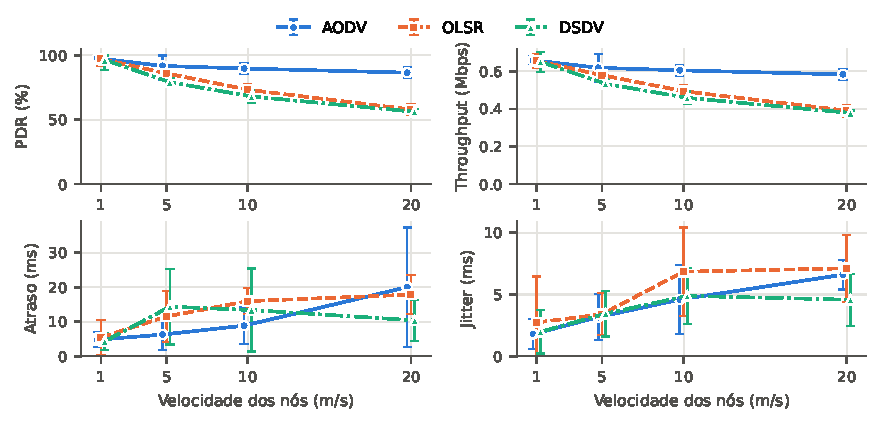
\includegraphics[width=\textwidth]{figuras/fig_base.pdf}
\caption{Métricas por velocidade (média de 5 execuções; barras: IC 95\%)}
\label{fig:base}
\end{figure}

\textbf{PDR e throughput.} A 1\,m/s os três protocolos empatam, com cerca de 97\% de
entrega. O aumento da velocidade reduz o PDR em todos, mas em intensidades muito
diferentes: de 1 para 20\,m/s o AODV perde 11 pontos percentuais, e OLSR e DSDV perdem
cerca de 40. A partir de 10\,m/s os intervalos de confiança do AODV não se sobrepõem aos
dos proativos. O throughput acompanha o PDR, como esperado em tráfego de taxa constante.
Não há ponto de ruptura brusco: em OLSR e DSDV a maior queda por m/s ocorre entre 1 e
5\,m/s e a degradação segue gradual.

\textbf{Explicação.} A diferença está no tempo que cada protocolo leva para perceber que
um enlace quebrou. O AODV do ns-3 usa o aviso de falha da camada de enlace e refaz a rota
em seguida. O OLSR só descarta um vizinho depois de 6\,s sem HELLO, e o DSDV anuncia
tabelas a cada 15\,s. A 20\,m/s um nó percorre o alcance de 197\,m em cerca de 10\,s, tempo
da mesma ordem desses temporizadores, de modo que os proativos encaminham muitos pacotes
por rotas que já não existem. Dois dados do experimento apoiam essa leitura. O tráfego de controle do AODV dobra de 1 para 20\,m/s (de 10,8 para 21,5\,kbps),
enquanto o de OLSR e DSDV cresce pouco. E os pacotes entregues por OLSR e DSDV a 20\,m/s
percorrem menos saltos (1,4 e 1,3, contra 1,7 no AODV), sinal de que as rotas longas são
as que mais falham. O resultado concorda com \cite{broch1998} e \cite{johansson1999}.

\textbf{Atraso e jitter.} As duas métricas crescem com a velocidade, mas a variação entre
execuções é grande e os intervalos se sobrepõem: no AODV a 20\,m/s, duas execuções têm
atraso de 35\,ms e três ficam entre 8 e 11\,ms. Além disso, as duas métricas só consideram
pacotes entregues, o que favorece quem perde os pacotes das rotas longas. O efeito da
mobilidade, portanto, não é percebido igualmente: é claro em PDR e throughput e
inconclusivo, entre protocolos, em atraso e jitter.

A Figura~\ref{fig:comparativo} compara os protocolos a 20\,m/s, condição escolhida por ser
a de maior mobilidade e a que mais separa os protocolos.

\begin{figure}[ht]
\centering
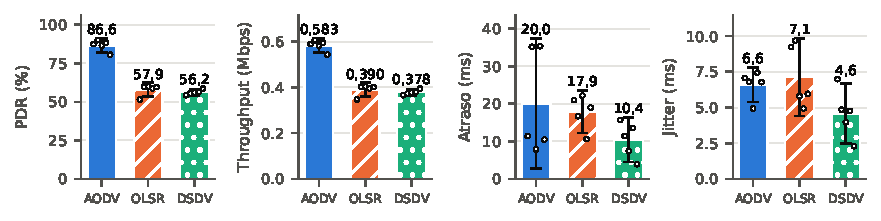
\includegraphics[width=\textwidth]{figuras/fig_comparativo.pdf}
\caption{Comparativo a 20\,m/s (barra: média; haste: IC 95\%; pontos: execuções)}
\label{fig:comparativo}
\end{figure}

\textbf{Variável adicional.} A Figura~\ref{fig:extensao} mostra o PDR para cada quantidade
de nós. A tendência do experimento-base se confirma: em todas as densidades o PDR de OLSR e
DSDV cai com a velocidade. A densidade, porém, muda a distância entre os protocolos. A
20\,m/s, de 20 para 40 nós, OLSR e DSDV sobem de cerca de 57\% para 65\%, e o AODV desce
de 86,6\% para 79,7\%. A 1\,m/s com 40 nós a ordem se inverte: o AODV entrega 86,0\% e os
proativos mais de 96\%. O motivo é o custo da descoberta de rotas por difusão, que cresce
com o número de vizinhos: a 10\,m/s o tráfego de controle do AODV passa de
16\,kbps com 20 nós para 101\,kbps com 40, contra 48\,kbps do OLSR e 57\,kbps do DSDV. Com
10 nós a rede é esparsa e a variação é muito grande (a 1\,m/s, PDR de 84\% $\pm$ 27 no
AODV), pois em algumas execuções há pares sem caminho por boa parte do tempo.

\begin{figure}[ht]
\centering
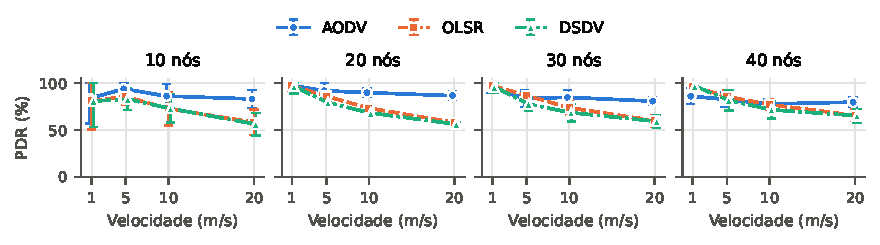
\includegraphics[width=\textwidth]{figuras/fig_extensao.pdf}
\caption{PDR em função da velocidade para 10, 20, 30 e 40 nós (barras: IC 95\%)}
\label{fig:extensao}
\end{figure}

\section{Conclusão}

No cenário simulado, o aumento da mobilidade reduz a entrega de pacotes nos três
protocolos, mas o reativo é bem menos afetado: a 20\,m/s o AODV entrega 86,6\% dos
pacotes, contra 57,9\% do OLSR e 56,2\% do DSDV. A baixa velocidade os três são
equivalentes. A mobilidade também eleva atraso e jitter, sem diferença conclusiva entre
protocolos. Redes mais densas ajudam os proativos e encarecem a descoberta de rotas do
AODV, a ponto de inverter a ordem em uma rede densa e quase parada.

Essas conclusões valem para os parâmetros padrão dos protocolos no ns-3.48, com cinco
repetições, propagação em espaço livre e Random Waypoint, modelo que concentra os nós no
centro da área \cite{camp2002}. Como trabalhos futuros, sugerem-se mais repetições, o
ajuste dos temporizadores dos protocolos proativos e outros modelos de mobilidade e de
propagação.

\bibliographystyle{sbc}
\bibliography{referencias}

\end{document}
